\documentclass[11pt]{article}

% Other packages for formatting
\usepackage[margin=1in]{geometry}
\usepackage{setspace}
\linespread{1.05}
% \onehalfspacing
\usepackage{fancyhdr}
\usepackage{graphicx}             % For including images
\usepackage{titlesec}             % For customizing section titles

\usepackage{amsmath, physics, amssymb}

% Set up the custom page style for the first page
\fancypagestyle{firstpagestyle}{
    \fancyhf{} % Clear all headers and footers
    \fancyhead[L]{\LARGE \textbf{Research Statement}}
    \fancyhead[R]{\Large \href{https://www.mathisgerdes.com}{\textbf{Mathis Gerdes}}}
    \renewcommand{\headrulewidth}{0pt} % Remove the default header rule
    \fancyfoot[C]{- {\thepage} -}
}

% Regular page style for the rest of the document
\pagestyle{fancy}
\fancyhf{} % Clear all headers and footers
\fancyhead[L]{\textbf{Research Statement}} % Regular header on subsequent pages
\fancyhead[R]{\textbf{Mathis Gerdes}}
\fancyfoot[C]{- {\thepage} -}

\usepackage{xcolor}
\definecolor{royalblue}{rgb}{0.2, 0.3, 0.7} % Adjust the RGB values for your preferred shade of blue
\usepackage[colorlinks=true, linkcolor=royalblue, urlcolor=royalblue, citecolor=royalblue]{hyperref}
\usepackage[colorlinks=true, linkcolor=royalblue, urlcolor=royalblue, citecolor=royalblue]{hyperref}

\usepackage{parskip}
\usepackage[sort&compress,numbers]{natbib}
\setlength{\bibsep}{2pt}

% Title information
\title{}
\author{}
\date{}

\begin{document}
\thispagestyle{firstpagestyle}


My research seeks to address complex questions in quantum field theory and string theory by pioneering computational and AI techniques, enabling new insights into non-perturbative regimes.
My experience spans machine learning approachees in lattice quantum chromodynamics (QCD) and string compactifications, where sophisticated tools are essential to push forward theoretical insights.

The Infosys-Cambridge AI Lab's focus on simulation-based approaches and theoretical machine learning aligns closely with my expertise.
My work spans AI-driven methods for geometry in string theory, lattice quantum field theory, foundational AI frameworks, and simulation-based inference.
I aim to contribute to the lab's goals by pushing forward the mathematical and computational boundaries of these fields.

\paragraph{\textit{{Calabi-Yau Metrics.}}}
Calabi-Yau manifolds play a crucial role in string compactifications.
Their geometric structure encoded in the metric is not known analytically, but is required for example to determine the Yukawa couplings of the low-energy effective theory.
This led me to devise novel machine learning methods to approximate Ricci-flat metrics on these manifolds.
By expressing a spectral ansatz that inherently guarantees important differential properties as a trainable neural network, I achieved higher accuracies than established methods more efficiently by simultaneously learning their moduli dependence.

This achievement was made possible by my efficient numerical implementation of intricate mathematical structures such as sections of holomorphic line bundles on complex projective spaces, metrics in local coordinate patches and derived geometric properties like the Ricci curvature.
Building on initial work during my MSc in theoretical and mathematical physics at the LMU Munich, I have since published a library of these computational methods \cite{gerdes2023CYJAXPackage} and co-authored an influential article explaining different machine learning approaches to this problem in collaboration with international collaborators \cite{anderson2021ModulidependentCalabiYau}.

\textbf{Future Directions:}
A rich space of mathematical constructions of Calabi-Yau manifolds remains to be explored, including the extension of my spectral method to complete intersection Calabi-Yau manifolds.
Additionally, it would be interesting to explore how incorporating advances in symbolic AI could enhance the efficiency and interpretability of computational frameworks in Calabi-Yau geometry

The field of AI applications in string theory and mathematics is becoming increasingly rich.
In this context, it appears to me that the utilization of long-established ideas in metaheuristics such as particle swarm optimization, simulated annealing and evolutionary algorithms remain under-explored.

\paragraph{\textit{{Lattice Quantum Field Theory and Non-Perturbative QCD.}}}
Quantum chromodynamics in the non-perturbative regime remains one of the most challenging and important areas of theoretical physics.
Lattice QCD provides a powerful framework for exploring this regime, but computational limitations have historically restricted our ability to fully explore it.
In my research, I have pioneered continuous normalizing flows for learning the complex distributions arising in lattice quantum field theory. By building the symmetries of the discretized theory directly into a trainable ordinary differential equation that parametrizes the field transformations, I have demonstrated state of the art performance on scalar theories \cite{gerdes2023LearningLattice}.

Building on these advances, I have recently devised and implemented a flexible framework of equivariant continuous normalizing flows on matrix Lie groups (example in Figure \ref{fig:su3}).
In particular, I have applied this to define continuous gauge equivariant flows for pure Yang-Mills theories in two dimensions, achieving state of the art performance on SU(2) and SU(3) \cite{gerdes2024continuousGauge}.
% I have recently extended this work to gauge theories, developing flexible gauge-equivariant continuous flows.
This involved implementing an integration scheme for matrix group manifolds that facilitates efficient gradient computation by leveraging modern ML libraries, and designed a new gauge-equivariant ODE architecture. % that delivers state-of-the-art sampling quality.

\textbf{\color{royalblue}{Future Directions.}}
I will continue this work with my collaborators by addressing the problem of scaling up to larger lattice sizes, including exploring multi-scale generation, transfer learning, and the thermodynamic properties of these flows, as well as their deeper connection to the renormalization group (RG). Leveraging the structural overlap in mathematical concepts, I have also recently become excited about the prospect of combining my experience in the context of Calabi-Yau manifolds to improve sampling for $\mathbb{CP}^N$ models, which suffers from topological freezing.

\begin{figure}
    \centering
    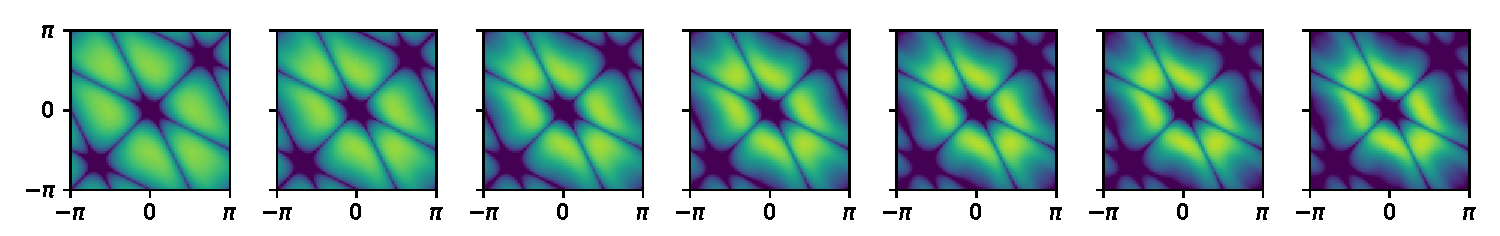
\includegraphics[width=\linewidth]{su3.pdf}
    \vspace{-25pt}
    \caption{\footnotesize Density of conjugation equivariant continuous flow on SU(3) in angular coordinates along flow time.}
    \label{fig:su3}
    \vspace{-10pt}
\end{figure}

\paragraph{\textit{{Physics for AI.}}}
Informed by my work on generative models for lattice quantum field theory, I have explored connections between RG and diffusion models.
This led me to developed a generalized RG-inspired framework for diffusion models \cite{gerdes2024gudgenerationunifieddiffusion}, in collaboration with Prof Max Welling, that enlarges the design space for diffusive processes and makes explicit its sequential nature.

\textbf{\color{royalblue}{Future Directions.}}
It is clear that notion of information and computation are foundational both to physics and machine learning.
Studying ML in the context of theoretical physics is thus bound to be fruitful in both directions, and I will continue exploring concrete ideas that have arisen from my work, including connections between generative models and thermodynamics, RG flows, and ODEs.

\paragraph{\textit{{Simulation based inference and statistics.}}}
Yet another example of interdisciplinary work I have enjoyed is in statistical data analysis and in particular simulation based inference, which incorporates machine learning to tackle large numbers of nuisance parameters that can arise from more faithful physical models.
In this context, I have developed an efficient simulator for stellar streams evolving in a gravitational background, to advance theoretical insight derived from astrophysical observations  \cite{alvey2023AlbatrossScalable}.
This led me to study theoretical statistics and differences between frequentist and Bayesian approaches in this field.
Having discovered an interesting dual point of view between these, I am presently studying optimization schemes that combine and unify notions from both frequentism and Bayesianism.


% \renewcommand{\refname}{}

% \vspace{15pt}
% \hrule
% \vspace{-35pt}
\bibliographystyle{abbrvnat-sorted}
{
    \small
    \bibliography{refs}
}

\end{document}
